\subsection{Step E. Explanation-generating search in IDP} 
A part of the holy grail challenge was not to just solve the puzzle from the natural language specification, but also to \emph{explain} how the solution was obtained, or rather, to explain how a human could obtain this solution as well. 

The idea of our explanation approach is that we will gradually fill the logigram grid with more and more information. The explanation is hence a series of reasoning steps, and at each step, information is added that can be obtained by reasoning on the clues and by using the partial solution obtained so far. 

\paragraph{Simple Explanations}
In order to make the explanations as simple as possible we order the reasoning steps (derivations) in the following way: 
\begin{itemize}
 \item Derivations that can be made without using any clues are always prioritized. These derivations are made solely using logigram axioms, such as the fact that all involved predicates are bijections as explained above. % (for instance, from the fact that the Englishman lives in the blue house, we can derive that he does not live in the red house, or from the fact that the Russian lives neither in the blue,red nor the green house, we can derive that he lives in the black house). 
 \item Next, derivations that require one or more clues are executed, where fewer clues are preferred. 
 \item Within both of the above classes, we always prioritize derivations that can be made by as little as possible information, that is, using as few as possible of the fields in the grid that have been filled already (see below for details on how to compute this).
\end{itemize}
It deserves to be noted that in the examples we encountered, it sufficed to only consider derivations that use at most one clue. This is probably due to puzzle designers making their puzzles easy enough. However, we can craft artificial examples in which that does not work, as illustrated next. 
\begin{example}
 Consider the following two clues of a logic puzzle. 
 \begin{quote}
  ``Either the Englishman lives in the red house with the fish, or he lives in the green house with the dog. '' \\
  ``If the Russian is a tea drinker, then the Englishman keeps a dog in the red house.'' 
 \end{quote}
%XXX \tias{No sigarette advertisement in our paper please...}
From these two clues, it follows that the Russian is not a tea drinker, but this can not be obtained by isolated reasoning over the two clues separately and at each step only deriving information that is present in a logic puzzle grid.  
\end{example}

\paragraph{Implementation}
% \todo{remove}
In order to implement this, we ensured that our automatic translation contains a separate logical theory for each clue, so that we can reason over the clues separately. For this, we made use of \idp's procedural interface (based on the lua scripting language) in which theories and structures are first-order citizens, and of the built-in inference methods described above. 
% We furthermore used the following built-in inference mechanisms: 
% \begin{itemize}
%  \item \textbf{optimalpropagate(T,S)} This inference method takes as input a theory $T$ and a partial structure $S$, it returns the most precise partial structure $S$ that approximates all models of $T$ that expand $S$
%  \item \textbf{unsatstructure(T,S,V)} This inference methods takes as input a theory $T$ and a structure $S$ such that $T$ has no models that expand $S$ (and optionally a vocabulary $V$). It returns structure $S'$ less precise than $S$, but equal to $S$ outside $V$ such that $T$ still has no models more precise than $S'$; furthermore the returned structured is minimally precise among such structures. Intuitively, this inference methods finds the reason for an inconsistency: it explains why there are no models of $T$ expanding $S$ by identifying a minimal set of assumptions in $S$ that cause the lack of models. 
%  Internally, this is implemented using unsatisfiable core extraction \cite{conf/sat/LynceM04}. 
% \end{itemize}
% 

These methods are used as follows. Our procedure maintains a partial structure $S$ representing the current state of the grid.\footnote{Since such a structure interprets all the predicates, which are binary relations between two types, a partial structure indeed corresponds nicely to a partially filled grid.} 
At each point in time, for all sets of clues of a given size $n$ (starting with $n=0$), all consequences (value assignments) of the conjunction of this set of clues are computed with \textbf{optimalpropagate}. 
If there are no consequences, the same is repeated for a greater $n$. 
For each of the consequences, a minimal set of facts from the partial structure $S$ that entail this consequence is computed using \textbf{unsatstructure} (this is done by making the consequence false in $S$ and using $V$ to disallow changing this consequence in the outcome of the unsatstructure-call). 
The result is a set of pairs $(S',\mathit{clues},\mathit{fact})$ where $S'$ is a substructure of $S$ such that from the set of clues $\mathit{clues}$ and $S'$ the fact $\mathit{fact}$ followed; for all computed facts.  %\tias{can be multiple?} \bart{Multiple what? Multiple clues? facts? To be precise about facts: yes, multiple facts can follow from the same clue and S'. What I actually do is: for each fact, compute a different $S'$ (this S' is only guaranteed to be subset-minimal, not cardinality minimal, and is determined based on the search path followed by the solver, hence, a different S' might be detected for  different facts... I then pick a smallest S' from which \emph{some fact} can be propagated and simply compute \emph{everything} that can be propagated from that S' and propagate it at once. Should I detail this a bit more? } \tias{No, but in future we should have pseudo-code for this part
Among those, a cardinality-minimal set $S'$ is selected and its propagation is executed and added to the list of derivations that make up the explanation.
Afterwards, the procedure starts over with $n=0$. 

%\todo{discuss variants? We have quite some implemented... } 
%\todo{discuss optimizations}

\paragraph{Propagation Strength}
One important thing to note here is that when we apply propagation, we do not do it on a theory that \emph{only} contains the clues in question. Instead, that theory always also contains all logigram axioms (bijections, transitivity, etcetera). 
The reason is that clues by themselves rarely propagate. To illustrate this, let us consider some examples. 
\begin{example}
 Consider the clue ``The patient who was prescribed enalapril is not Heather''. If one were to manually translate this clue into first-order logic over the given vocabulary, one would probably come up with: 
 \begin{align}\lnot \mathit{prescribed}(heather,enalapril).\label{eq:heather:easy}\end{align}
 However, our automatic parsing method makes an explicit mention of ``the person who'' in the form of a logic variable and instead produces 
 \begin{align}
  \exists p: prescribed(p,enalapril) \land p \neq heather.\label{eq:heather:produced}
\end{align}
If the system were given the clue ``Heather was not prescribed enalapril'', the system would find \eqref{eq:heather:easy}.
Equations \eqref{eq:heather:easy} and \eqref{eq:heather:produced} are not equivalent and in fact from \eqref{eq:heather:produced} it does not follow that heather is not prescribed enalapril. That is... unless the fact that there is exactly one person who is prescribed enalapril is taken into account. In conjunction with the theory stating that all predicates are bijections, these two equations are equivalent. 
% 
% This sentence is not equivalent to the first 
% 
\end{example}

\begin{example}
 Consider the clue ``The owner of the lime house was prescribed enalapril'', which is translated into first-order logic as:
 \begin{align}
\exists o: lives\_in(o,lime) \land prescribed(o,enalapril).   \label{eq:lime}
 \end{align}
 This clue actually gives information about the relation between houses and medication. However, it is clear that from \eqref{eq:lime} alone we cannot propagate such information: it does not even mention the predicate that links houses and medications. 
 However, in combination with the transitivity and bijection axioms, we can propagate that 
 \[\lnot used\_in(enalapril,lime).\qedhere\]
\end{example}

\subsection{F. Visualisation of the explanation}
We explored two different possibilities to present this explanation to humans. 
The first was generating natural language sentences of the form 
``From the clue(s) $\langle$clue$\rangle$ and the fact that $\langle$assumptions$\rangle$, it follows that $\langle$conclusions$\rangle$.''
However, in our experience, as soon as there are a couple of assumptions involved, this kind of sentence easily becomes hard to read and understand. Furthermore, it is not always easy to create these sentences: if the input does not mention a name for the relation between medication and houses, how can we express that enalapril is \emph{not used in} the lime house? 
There are two possibilities to do that, the first is using a generic verb such as ``associated with'' (rendering boring sentences); the second is avoiding the relation and for instance writing ``the user of enalapril does not live in the lime house''. 

Overall, we were not satisfied with the outcome of this first approach, which is why we implemented a different way to present the explanation process to the user, namely by means of a visualisation. To represent our derivations, we make use of the standard grid in logic puzzles. In each step, we indicate which clue(s) are used, highlight all cells used for the propagation in blue and all conclusions in green. 
The user can then navigate through the reasoning process by means of ``next'' and ``previous'' buttons. 

Figure \ref{fig:screenshot} contains a screenshot of this explanation process. 
It displays a partially filled grid, in which checkmarks represent that something is derived to be true and minus signs that it is false. 
In this specific frame, we can see that the clue ``Roxanne is 2 years younger than the Kansas native'' is used, together with the previously derived knowledge (highlighted in orange) that the Kansas native is not 111 years old, we can derive (highlighted in blue) that Roxanne is not 109 years old.

\begin{figure}
 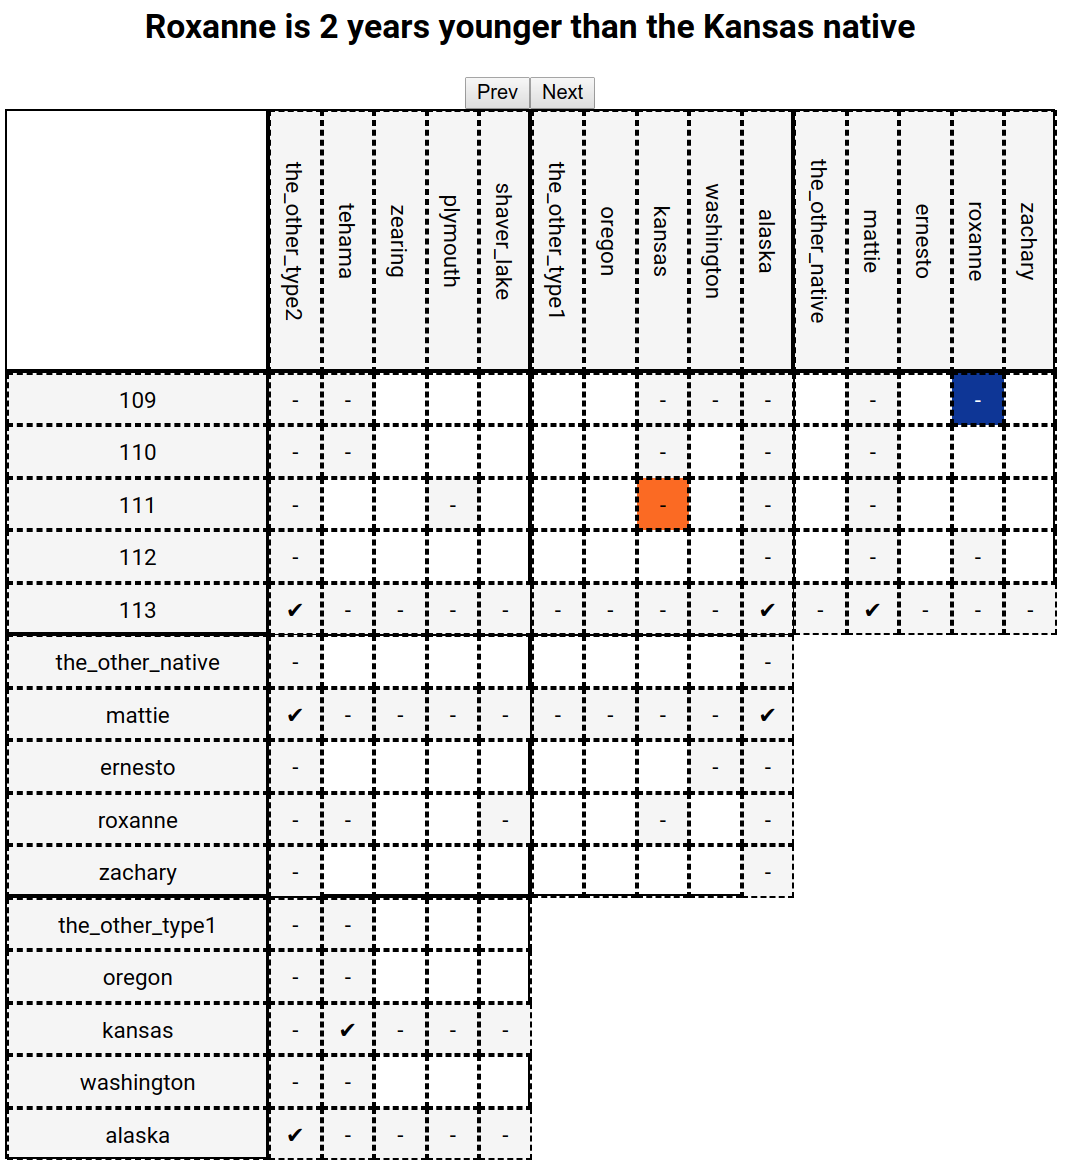
\includegraphics[width=\columnwidth]{fig/screenshot.png}
 \caption{Screenshot of the visualization.}
 \label{fig:screenshot}
\end{figure}




% 
% \todo{Something about the visualisation:
% Possibilities/Difficulties with NL generation (non-existing verbs for instance)}
